\chapter{Арга зүй ба системийн зохиомж}

% ============================================================
% Section 1: Хөгжүүлэлтийн төлөвлөгөө
% ============================================================
\section{Хөгжүүлэлтийн төлөвлөгөө}
Хөгжүүлэлтийн ажлыг Iterative (Давталттай) аргачлалаар гүйцэтгэсэн бөгөөд доорх үе шатуудад хуваав:
\begin{enumerate}
    \item \textbf{I үе шат}: Суурь өгөгдлийн сангийн өргөтгөл болон тогтмол илэрхийллийн шүүлтүүрийн алгоритм хөгжүүлэлт.
    \item \textbf{II үе шат}: Хавтас удирдлагын систем болон шудрах үйлдлүүдийн UI хөгжүүлэлт.
    \item \textbf{III үе шат}: Нугалдаг төхөөрөмжийн дасан зохицох харагдац болон тасралтгүй байдлын логик.
    \item \textbf{IV үе шат}: Гүйцэтгэлийн оновчлол, тест ба чанарын баталгаажуулалт.
\end{enumerate}

Хөгжүүлэлтийн явцад Git-ийн ``Feature Branch'' стратегийг~\cite{vincent_git} ашиглаж, долоо хоног бүр явцын түүхийг баталгаажуулсан.

% ============================================================
% Section 2: Хэрэглээний тохиолдлын шинжилгээ
% ============================================================
\section{Хэрэглээний тохиолдлын шинжилгээ}
Системийн функционал шаардлагуудыг хэрэглэгчийн үйлдэл бүрээр нарийвчлан тодорхойлохын тулд хэрэглээний тохиолдлын диаграммыг (Зураг~\ref{fig:usecase_diag}) боловсруулав.

\begin{figure}[H]
    \centering
    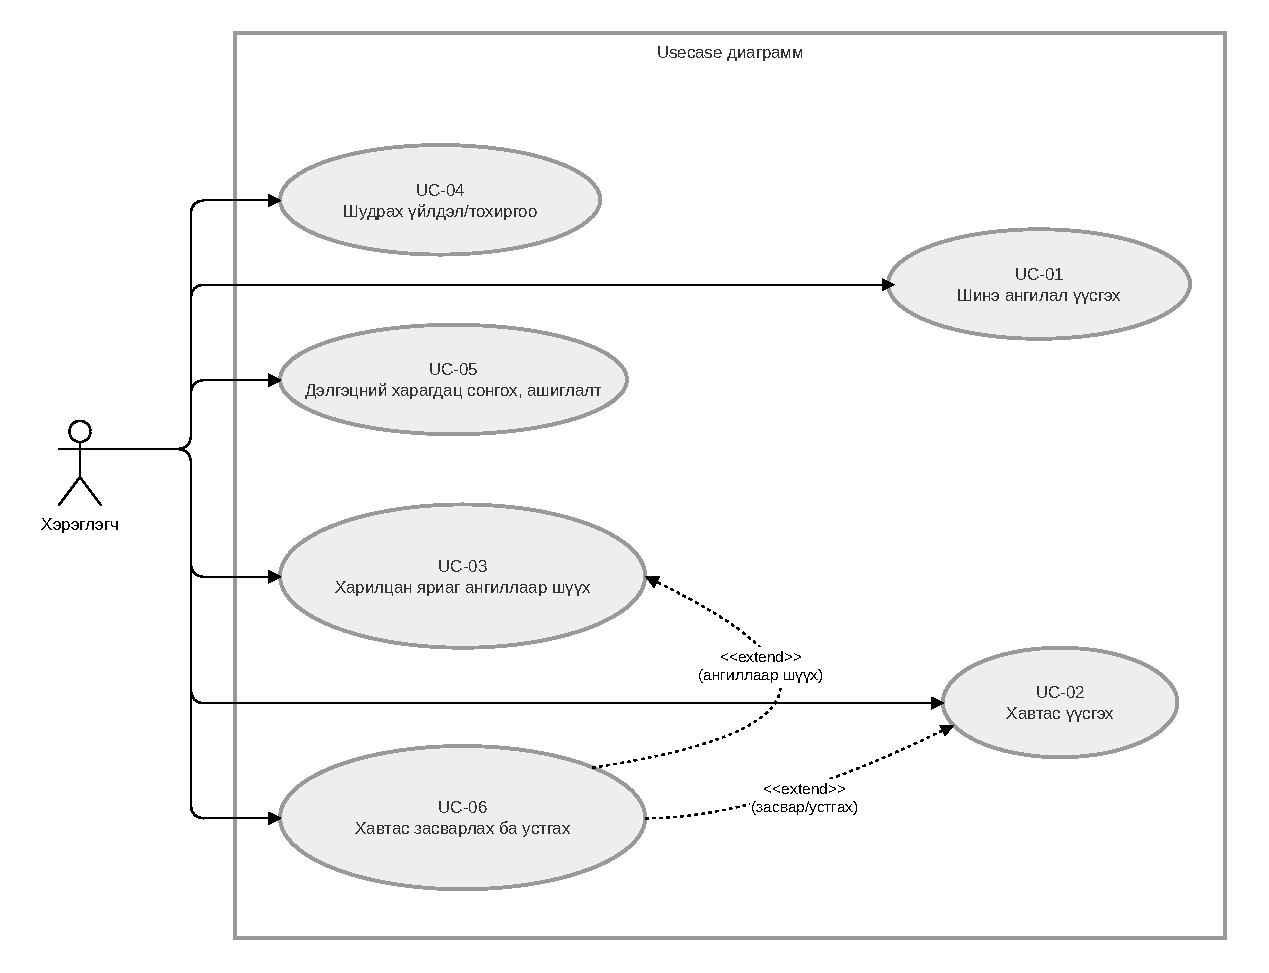
\includegraphics[width=0.85\textwidth]{Diagrams/usecase_diagram}
    \caption{Системийн хэрэглээний тохиолдлын диаграмм}
    \label{fig:usecase_diag}
\end{figure}

Дээрх диаграммд тусгагдсан үндсэн үйлдлүүдийн ажлын урсгал болон нөхцөлүүдийг дараах хүснэгтүүдээр дэлгэрэнгүй тайлбарлав.

% Хэрэглээний тохиолдол 1: Шошго үүсгэх
\begin{longtable}{|l|p{10.5cm}|}
    \caption{Хэрэглээний тохиолдол 1: Шошго үүсгэх} \label{tab:uc_create_category} \\
    \hline
    \textbf{ID / Нэр} & UC-01 / Шинэ шошго үүсгэх \\ \hline
    \textbf{Товч тайлбар} & Хэрэглэгч зурвас шүүх шинэ дүрэм (шошго) үүсгэж, нэр, өнгө болон шүүлтүүрүүдийг тохируулна. \\ \hline
    \textbf{Үйлдэгч} & Хэрэглэгч \\ \hline
    \textbf{Өмнөх нөхцөл} & Хэрэглэгч ``Шошго удирдах'' дэлгэцийг нээсэн байна. \\ \hline
    \textbf{Ажлын урсгал} &
    1. Хэрэглэгч ``+'' товчийг дарж үүсгэх цонхыг нээнэ. \newline
    2. Шошгоны нэрийг оруулж, жагсаалтаас өнгө сонгоно. \newline
    3. Шүүлтүүрийн төрлийг сонгоно: \newline
    \hspace{0.5cm} 3.1. Энгийн үг оруулах бол ``Энгийн үг нэмэх'' талбарт бичнэ. \newline
    \hspace{0.5cm} 3.2. Тогтмол илэрхийлэл (Regex) ашиглах бол дүрс дээр дарж паттерн оруулна. \newline
    4. Оруулсан өгөгдлийг шалгаж ``OK'' товчийг дарна. \\ \hline
    \textbf{Альтернатив} & Хэрэглэгч ``Cancel'' дарвал өөрчлөлт хадгалагдахгүй. Буруу тогтмол илэрхийллийн паттерн оруулбал систем алдаа заана. \\ \hline
    \textbf{Дараах нөхцөл} & Шинэ шошго баазад хадгалагдаж, зурвасууд шууд ангилагдана. \\ \hline
\end{longtable}

\vspace{1em}

% Хэрэглээний тохиолдол 2: Хавтас үүсгэх
\begin{longtable}{|l|p{10.5cm}|}
    \caption{Хэрэглээний тохиолдол 2: Хадгалсан харагдац (Хавтас) үүсгэх} \label{tab:uc_create_folder} \\
    \hline
    \textbf{ID / Нэр} & UC-02 / Хавтас үүсгэх \\ \hline
    \textbf{Товч тайлбар} & Хэрэглэгч өөрийн хэрэгцээнд тохирсон зурвасын харагдац (Хавтас) үүсгэж, доод навигацийн цэсэнд нэмнэ. \\ \hline
    \textbf{Үйлдэгч} & Хэрэглэгч \\ \hline
    \textbf{Ажлын урсгал} &
    1. Баруун дээд цэснээс ``Хавтас'' -> ``Харагдац үүсгэх'' сонгоно. \newline
    2. Хавтасны нэрийг бичиж, харагдах байрлал (index) болон өнгийг тодорхойлно. \newline
    3. ``OK'' товчийг дарж баталгаажуулна. \\ \hline
    \textbf{Дараах нөхцөл} & Шинэ хавтас доод навигацийн цэсэнд нэмэгдэж, хэрэглэгч тухайн хавтас руу автоматаар шилжинэ. \\ \hline
\end{longtable}

\vspace{1em}

% Хэрэглээний тохиолдол 3: Шошгоор шүүх
\begin{longtable}{|l|p{10.5cm}|}
    \caption{Хэрэглээний тохиолдол 3: Шошгоор шүүх} \label{tab:uc_filter_category} \\
    \hline
    \textbf{ID / Нэр} & UC-03 / Харилцан яриаг шошгоор шүүх \\ \hline
    \textbf{Товч тайлбар} & Хэрэглэгч үүсгэсэн хавтас доторх харилцан яриануудыг нэг болон хэд хэдэн шошгоор (Tag) шүүж харна. \\ \hline
    \textbf{Ажлын урсгал} &
    1. Хайх талбарын хажууд байрлах шүүлтүүрийн товчийг дарна. \newline
    2. Гарч ирэх жагсаалтаас нэг болон түүнээс дээш шошгыг сонгоно. \newline
    3. ``OK'' товчийг дарахад систем сонгосон шошгонд таарсан зурвасуудыг харуулна. \\ \hline
    \textbf{Дараах нөхцөл} & Жагсаалт шинэчлэгдэж, шүүлтийн төлөв хадгалагдана. \\ \hline
\end{longtable}

\vspace{1em}

% Хэрэглээний тохиолдол 4: Шудрах үйлдэл
\begin{longtable}{|l|p{10.5cm}|}
    \caption{Хэрэглээний тохиолдол 4: Шудрах үйлдлийн тохиргоо} \label{tab:uc_swipe_actions} \\
    \hline
    \textbf{ID / Нэр} & UC-04 / Шудрах үйлдлийн тохиргоо \\ \hline
    \textbf{Товч тайлбар} & Харилцан ярианы жагсаалтад зүүн эсвэл баруун тийш шудрахад хийгдэх үйлдлийг хэрэглэгч өөрөө сонгоно. \\ \hline
    \textbf{Ажлын урсгал} &
    1. Програмын ерөнхий тохиргооноос ``Шудрах үйлдэл'' хэсгийг нээнэ. \newline
    2. ``Эхнээс нь шудрах'' эсвэл ``Төгсгөлөөс нь шудрах'' сонголтыг дарна. \newline
    3. Боломжит үйлдлүүдээс (Устгах, Архивлах, Уншсан болгох г.м) нэгийг сонгоно. \\ \hline
    \textbf{Дараах нөхцөл} & Сонгосон үйлдэл тэр даруй хадгалагдаж, жагсаалт дээр ажиллаж эхэлнэ. \\ \hline
\end{longtable}

\vspace{1em}

% Хэрэглээний тохиолдол 5: Дэлгэцийн горим
\begin{longtable}{|l|p{10.5cm}|}
    \caption{Хэрэглээний тохиолдол 5: Дэлгэцийн харагдацын горим} \label{tab:uc_screen_view} \\
    \hline
    \textbf{ID / Нэр} & UC-05 / Screen View Mode сонгох \\ \hline
    \textbf{Товч тайлбар} & Нугалдаг төхөөрөмж эсвэл таблет дээр жагсаалт болон дэлгэрэнгүй хэсгийг хэрхэн харуулахыг тохируулна. \\ \hline
    \textbf{Ажлын урсгал} &
    1. Тохиргоо цэсний ``View mode'' хэсэгт орно. \newline
    2. ``Auto'', ``Single'', эсвэл ``Separated'' горимуудаас нэгийг сонгоно. \newline
    3. ``Auto'' горимд систем дэлгэцийн төлөвийг (Дэлгэц хаалттай/нээлттэй) мэдэрч автоматаар шилжинэ. \\ \hline
    \textbf{Дараах нөхцөл} & Програмын үндсэн дэлгэцийн бүтэц (layout) сонгосон горимын дагуу шинэчлэгдэнэ. \\ \hline
\end{longtable}

\vspace{1em}

% Хэрэглээний тохиолдол 6: Хавтас засварлах
\begin{longtable}{|l|p{10.5cm}|}
    \caption{Хэрэглээний тохиолдол 6: Хавтас засварлах ба устгах} \label{tab:uc_edit_folder} \\
    \hline
    \textbf{ID / Нэр} & UC-06 / Хавтас засах эсвэл устгах \\ \hline
    \textbf{Товч тайлбар} & Өмнө үүсгэсэн хавтасны мэдээллийг шинэчлэх эсвэл системээс бүрмөсөн устгана. \\ \hline
    \textbf{Ажлын урсгал} &
    1. Доод навигацийн цэс дээрх хавтасны дүрс дээр удаан дарна. \newline
    2. Мэдээллийг (нэр, өнгө, байрлал) засаад ``OK'' дарах эсвэл ``Delete'' товчийг сонгоно. \newline
    3. Устгах үйлдэл дээр систем дахин баталгаажуулалт асууна. \\ \hline
    \textbf{Дараах нөхцөл} & Өөрчлөлт хадгалагдах эсвэл хавтас навигацийн цэснээс алга болж хэрэглэгч үндсэн харагдац руу шилжинэ. \\ \hline
\end{longtable}


% ============================================================
% Section 3: Системийн архитектур
% ============================================================
\section{Системийн архитектур}
Системийн ерөнхий архитектурыг Зураг \ref{fig:architecture} уламжлалт 3 давхаргат (3-Layer Architecture) бүтцээр зохиомжилсон бөгөөд энэ нь өгөгдлийн, логик болон хэрэглэгчийн харилцах цонхны хэсгүүдийг бие даан хөгжүүлэх, турших боломжийг олгосон.

\begin{itemize}
    \item \textbf{Өгөгдлийн давхарга (Data Layer)}: Room Persistence Library ашиглан локал SQLite баазад зурвас, харилцан яриа болон ангиллын мэдээллийг хадгална.
    \item \textbf{Бизнес логикийн давхарга (Domain Layer)}: Тогтмол илэрхийллийн шүүлтүүрийн хөдөлгүүр болон хавтаслах системийн цөм логик байрлана.
    \item \textbf{Танилцуулга давхарга (Presentation Layer)}: XML View систем болон Jetpack Compose ашиглан хэрэглэгчийн харилцах цонхыг бүрдүүлнэ.
\end{itemize}

\begin{figure}[H]
    \centering
    
\includegraphics[width=0.55\textwidth]{Diagrams/architecture}
    \caption{Системийн ерөнхий бүтэц (Architecture Diagram)}
    \label{fig:architecture}
\end{figure}

% ============================================================
% Section 4: Өгөгдлийн сангийн зохиомж
% ============================================================
\section{Өгөгдлийн сангийн зохиомж}
Өгөгдлийн сангийн гол бүтэц, хүснэгт хоорондын холбоосыг ER диаграммаар Зураг~\ref{fig:erd} дээр үзүүлэв.

\begin{figure}[H]
    \centering
    
\includegraphics[width=0.55\textwidth]{Diagrams/erd}
    \caption{Өгөгдлийн сангийн ерөнхий бүтэц (ER Diagram)}
    \label{fig:erd}
\end{figure}

\begin{itemize}
    \item \textbf{Categories}: Ангиллын нэр, өнгө, дүрмийн тохиргоо хадгална.
    \item \textbf{Rules}: Түлхүүр үг болон тогтмол илэрхийллийн дүрэм, ангилалтай холбогдоно.
    \item \textbf{Харилцан яриа}: Харилцан ярианы ерөнхий мэдээлэл, ангиллын холбоос.
    \item \textbf{Messages}: Бодит зурвасын агуулга, илгээгч, огноо, харилцан ярианд хамаарал.
\end{itemize}

\subsection{Өгөгдлийн сангийн шинэчлэл}
Төслийн хүрээнд \texttt{MessagesDatabase}-ийн хувилбарыг 10-аас 13 болгон ахиулж, дараах өөрчлөлтүүдийг хийсэн:
\begin{itemize}
    \item \textbf{MIGRATION 10--11}: \texttt{categories} хүснэгтийг шинээр үүсгэж, \texttt{messages} болон \texttt{conversations} хүснэгтүүдэд ангиллын мэдээллийг хадгалах (\texttt{category}, \texttt{categoryId}) талбаруудыг нэмсэн.
    \item \textbf{MIGRATION 11-12}: Түлхүүр үг нь тогтмол илэрхийлэл (Regex) эсэхийг тодорхойлох \texttt{keywords\_is\_regex} баганыг нэмж, шүүлтийн логикийг өргөтгөсөн.
    \item \textbf{MIGRATION 12--13}: Шүүлтүүрийн логикийг илүү нарийвчлалтай болгох зорилгоор \texttt{categories} хүснэгтэд \texttt{plain\_keywords} болон \texttt{regex\_patterns} багануудыг шинээр нэмж, "Dual-mode" шүүлтийг зэрэг ажиллуулах нөхцөлийг бүрдүүлсэн.
\end{itemize}

\begin{figure}[H]
    \centering
    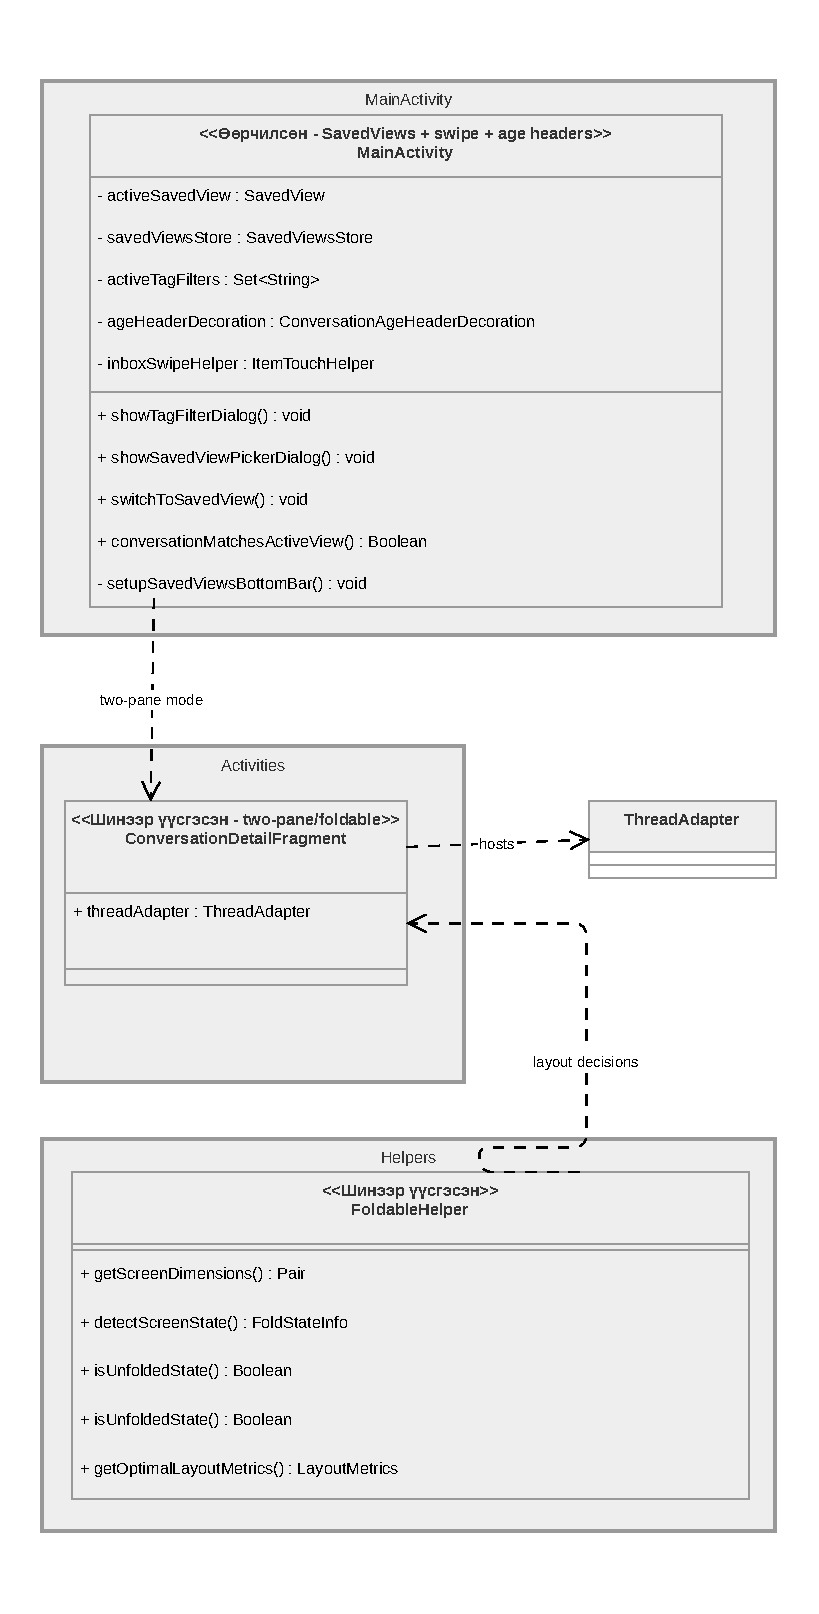
\includegraphics[width=0.9\textwidth]{Diagrams/class/database}
    \caption{Өгөгдлийн сангийн бүтэц болон DAO-ийн класс диаграмм}
    \label{fig:db_schema}
\end{figure}

% ============================================================
% Section 5: Нарийвчилсан зохиомж ба логик дараалал
% ============================================================
\section{Нарийвчилсан зохиомж ба Логик дараалал}
Системийн хамгийн чухал процесс болох ``Ангилал үүсгэх, түүний хэрэгжилт''-ийн логикийг UML Sequence диаграммаар (Зураг~\ref{fig:seq_diag}) харуулав. Диаграммд хэрэглэгчийн ангиллын нэр, өнгө болон түлхүүр үгсийг оруулах үйлдэл, өгөгдлийн сан руу хадгалах процесс, мөн тухайн ангиллын дагуу зурвасыг автоматаар ангилах үйл явцын урсгалыг харуулсан.

\begin{figure}[H]
    \centering
    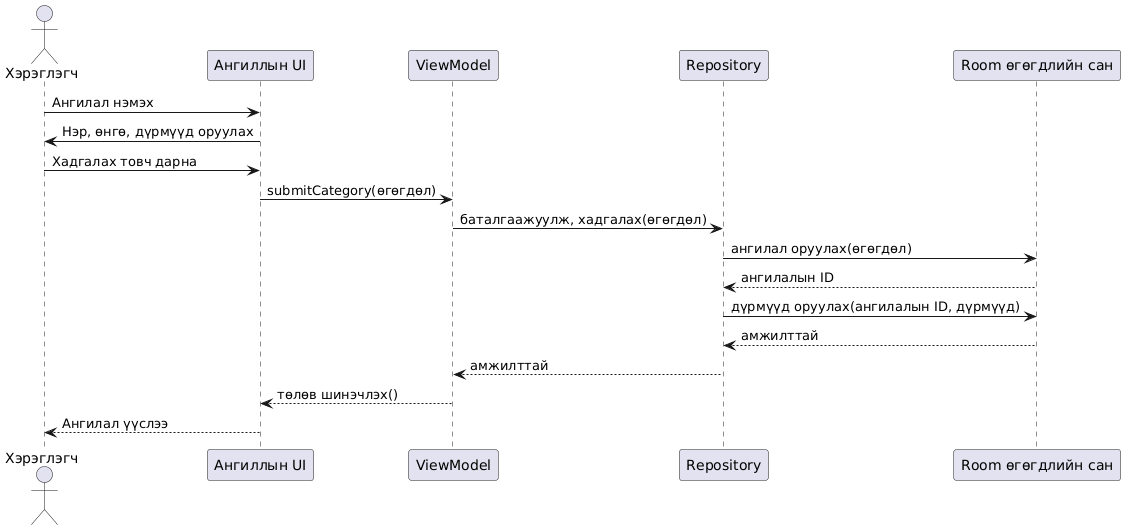
\includegraphics[width=0.85\textwidth]{Diagrams/sequence/category_sequence}
    \caption{Ангилал шинээр үүсгэх (Sequence Diagram)}
    \label{fig:seq_diag}
\end{figure}

Хавтас үүсгэх болон хадгалах логикийг дарааллын диаграммаар (Зураг~\ref{fig:seq_category}) харуулав. Хавтас үүсгэх, тохируулах үйлдэл төстэй бүтэцтэй бөгөөд өгөгдлийн нэгдсэн урсгал хэсэгт аль алинд ижилхэн процессуудыг агуулдаг тул нэг диаграммд цэнхэр өнгө бүхий хэсэгт нэгтгэн үзүүлэв. Улаан өнгөөр тэмдэглэсэн хэсэг нь ангиллын дүрмийн тохиргоонуудын нэг болох устгах үйлдлийг харуулсан.

\begin{figure}[H]
    \centering
    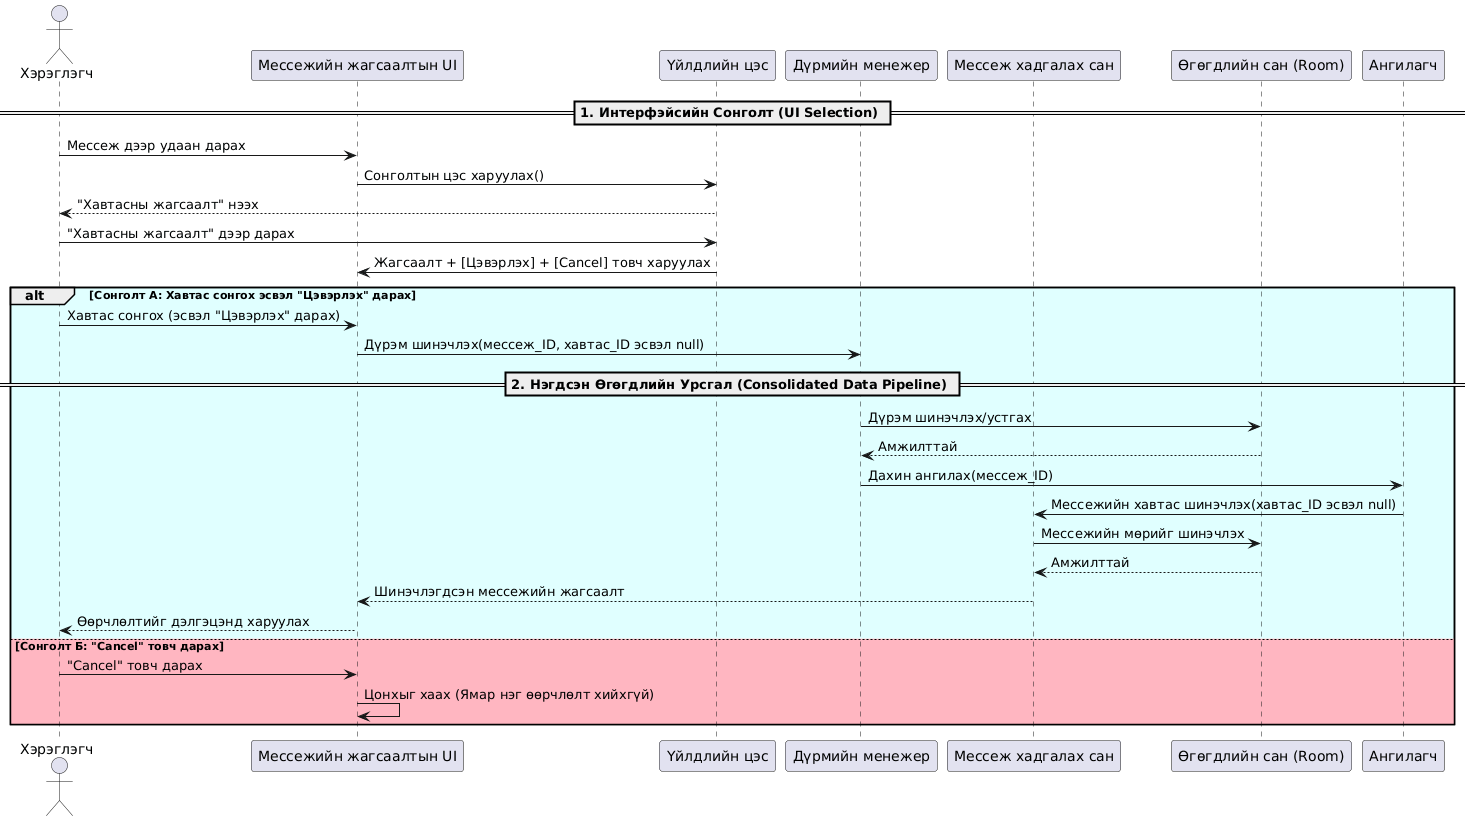
\includegraphics[width=0.85\textwidth]{Diagrams/sequence/assign_folder_sequence.png}
    \caption{Хавтас үүсгэх болон хадгалах дараалал (Sequence Diagram)}
    \label{fig:seq_category}
\end{figure}

Мөн харилцан яриан дээр удаан дарснаар гарч ирэх доод хэсгийн тохиргоо гарч ирж тэдгээрээс сонгох явцыг үйл ажиллагааны диаграммаар (Зураг~\ref{fig:act_diag}) дүрслэв. Хавтас оноохоос гадна бусад үндсэн үйлдлүүдийг (архивлах, устгах, уншсан төлөв солих) нэгтгэн харуулсан бөгөөд тэдгээр үйлдэлийг үр дүнг нарийн тайлбарлахгүйгээр үр дүнг төгсгөл хэсэг рүү шууд чиглүүлсэн.

\begin{figure}[H]
    \centering
    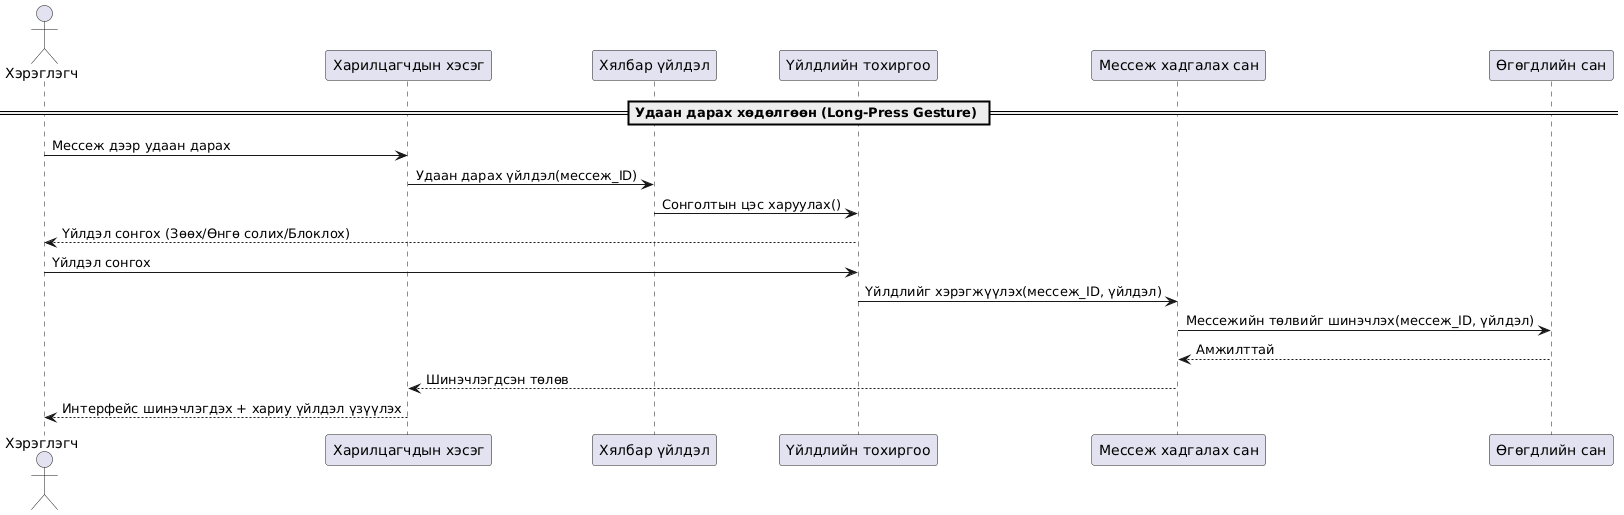
\includegraphics[width=0.85\textwidth]{Diagrams/sequence/long_press_sequence_diagram}
    \caption{Удаан дарж гарч ирэх туслах цэсний логик}
    \label{fig:act_diag}
\end{figure}

\section{Төслийн суурь бүтэц (Fossify Messages)}
Fossify Messages (мөн өмнөх Simple Mobile Tools) төслийн сангуудын бүтэц нь Android хөгжүүлэлтийн стандарт болон Separation of Concerns (үүрэг хариуцлагыг тусгаарлах) зарчмыг баримталдаг. Үндсэн хавтаснуудын үүргийг доор дэлгэрэнгүй тайлбарлав.

\begin{itemize}
    \item \textbf{activities/ (Presentation Layer)}: Энэ санд аппликейшны бүх дэлгэцүүд (UI screens) байрлана. Жишээ нь: \texttt{MainActivity} (мессежийн жагсаалт), \texttt{ThreadActivity} (тухайн харилцагчтай харилцсан түүх), \texttt{SettingsActivity}. Android-ийн ажиллах үндсэн цэгүүд энд байна.

    \item \textbf{adapters/ (UI Logic)}: Жагсаалттай ажилладаг классууд байрлана. \texttt{RecyclerView}-д өгөгдлийг (мессеж, харилцан яриа) хэрхэн харуулахыг зохицуулдаг. Жишээ нь: \texttt{ThreadAdapter} нь чат доторх мессеж бүрийн харагдах байдлыг удирддаг.

    \item \textbf{App.kt (Global Configuration)}: Аппликейшн ажиллахад хамгийн түрүүнд дуудагддаг класс. Энд глобал тохиргоонууд, Dependency Injection (DI)-ийн эхлэл, эсвэл өгөгдлийн сангийн бэлтгэл ажил хийгддэг.

    \item \textbf{databases/ (Data Layer)}: Room Persistence Library ашиглан локал өгөгдлийн сантай харьцах хэсэг. Энд \texttt{MessagesDatabase}, \texttt{ConversationsDao} зэрэг классууд байрлаж, SQLite-аас өгөгдөл унших, бичих үйлдлийг гүйцэтгэнэ.

    \item \textbf{dialogs/ (Reusable UI)}: Хэрэглэгчээс баталгаажуулалт авах, текст оруулах зэрэг жижиг цонхнууд (Pop-ups) энд байна. Жишээ нь: Мессеж устгах үеийн "Энэ үйлдлийг хийхдээ итгэлтэй байна уу?" цонх. Энэ нь элементийг дахин ашиглах \cite{design_patterns} зохистой арга юм.

    \item \textbf{extensions/ (Kotlin Power)}: Fossify төслүүдийн нэг онцлог бол Extension Functions маш их ашигладаг. Суурь классууд дээр (жишээ нь \texttt{Context}, \texttt{String}, \texttt{Long}) нэмэлт функц бичиж, кодыг эмх замбараагүй болохоос сэргийлдэг. Жишээ нь: \texttt{Long.formatDate()} гэх мэт.

    \item \textbf{helpers/ (Utilities)}: Туслах функцүүд болон тогтмол утгууд (Constants) байрлана. Мөн Prefs буюу хэрэглэгчийн тохиргоог (\texttt{SharedPrefs}) удирдах классууд энд байна.

    \item \textbf{interfaces/ (Abstraction)}: Классууд хоорондоо харилцах гүүр болох "Listener"-үүд байрлана. Жишээ нь: \texttt{RefreshMessagesListener} – өгөгдөл өөрчлөгдөхөд UI-г шинэчлэх үүрэгтэй.

    \item \textbf{messaging/ (Core Logic)}: Мессеж илгээх, хүлээн авах, SMS/MMS-ийн төрлийг тодорхойлох зэрэг системийн хамгийн чухал логикууд энд байрладаг. Энэ бол апп-ын "зүрх" нь юм.

    \item \textbf{models/ (Data Classes)}: Өгөгдлийн бүтэц буюу POJO классууд. Жишээ нь: \texttt{Message}, \texttt{Conversation}, \texttt{Contact} гэх мэт өгөгдлийн загварууд.

    \item \textbf{receivers/ (Android Components)}: Android системээс ирж буй дохиог (Broadcast) барьж авах хэсэг. Хамгийн чухал нь \texttt{SmsReceiver} буюу шинэ мессеж ирэхэд түүнийг барьж аваад апп-д мэдэгдэх үүрэгтэй.

    \item \textbf{services/ (Background Tasks)}: Ар талд (Background) ажиллах шаардлагатай ажлууд. Жишээ нь: Мессеж илгээх процесс дуустал ажиллах үйлчилгээ энд байна.

    \item \textbf{ui/ (Custom UI)}: Апп-д ашиглагдаж буй тусгайлан загварчилсан (Custom) View-үүд байрлана. Жишээ нь: Өнгө сонгогч, тусгай товчлуур гэх мэт.
\end{itemize}
% ============================================================
% Section 6: Класс диаграммууд
% ============================================================
\section{Системийн класс диаграммууд}

\subsection{Activity болон UI логикийн бүтэц}
Аппликейшны дэлгэцүүд болон тэдгээрийн хоорондын харилцан хамаарлыг Зураг~\ref{fig:class_activity}-д үзүүлэв.

\begin{figure}[H]
    \centering
    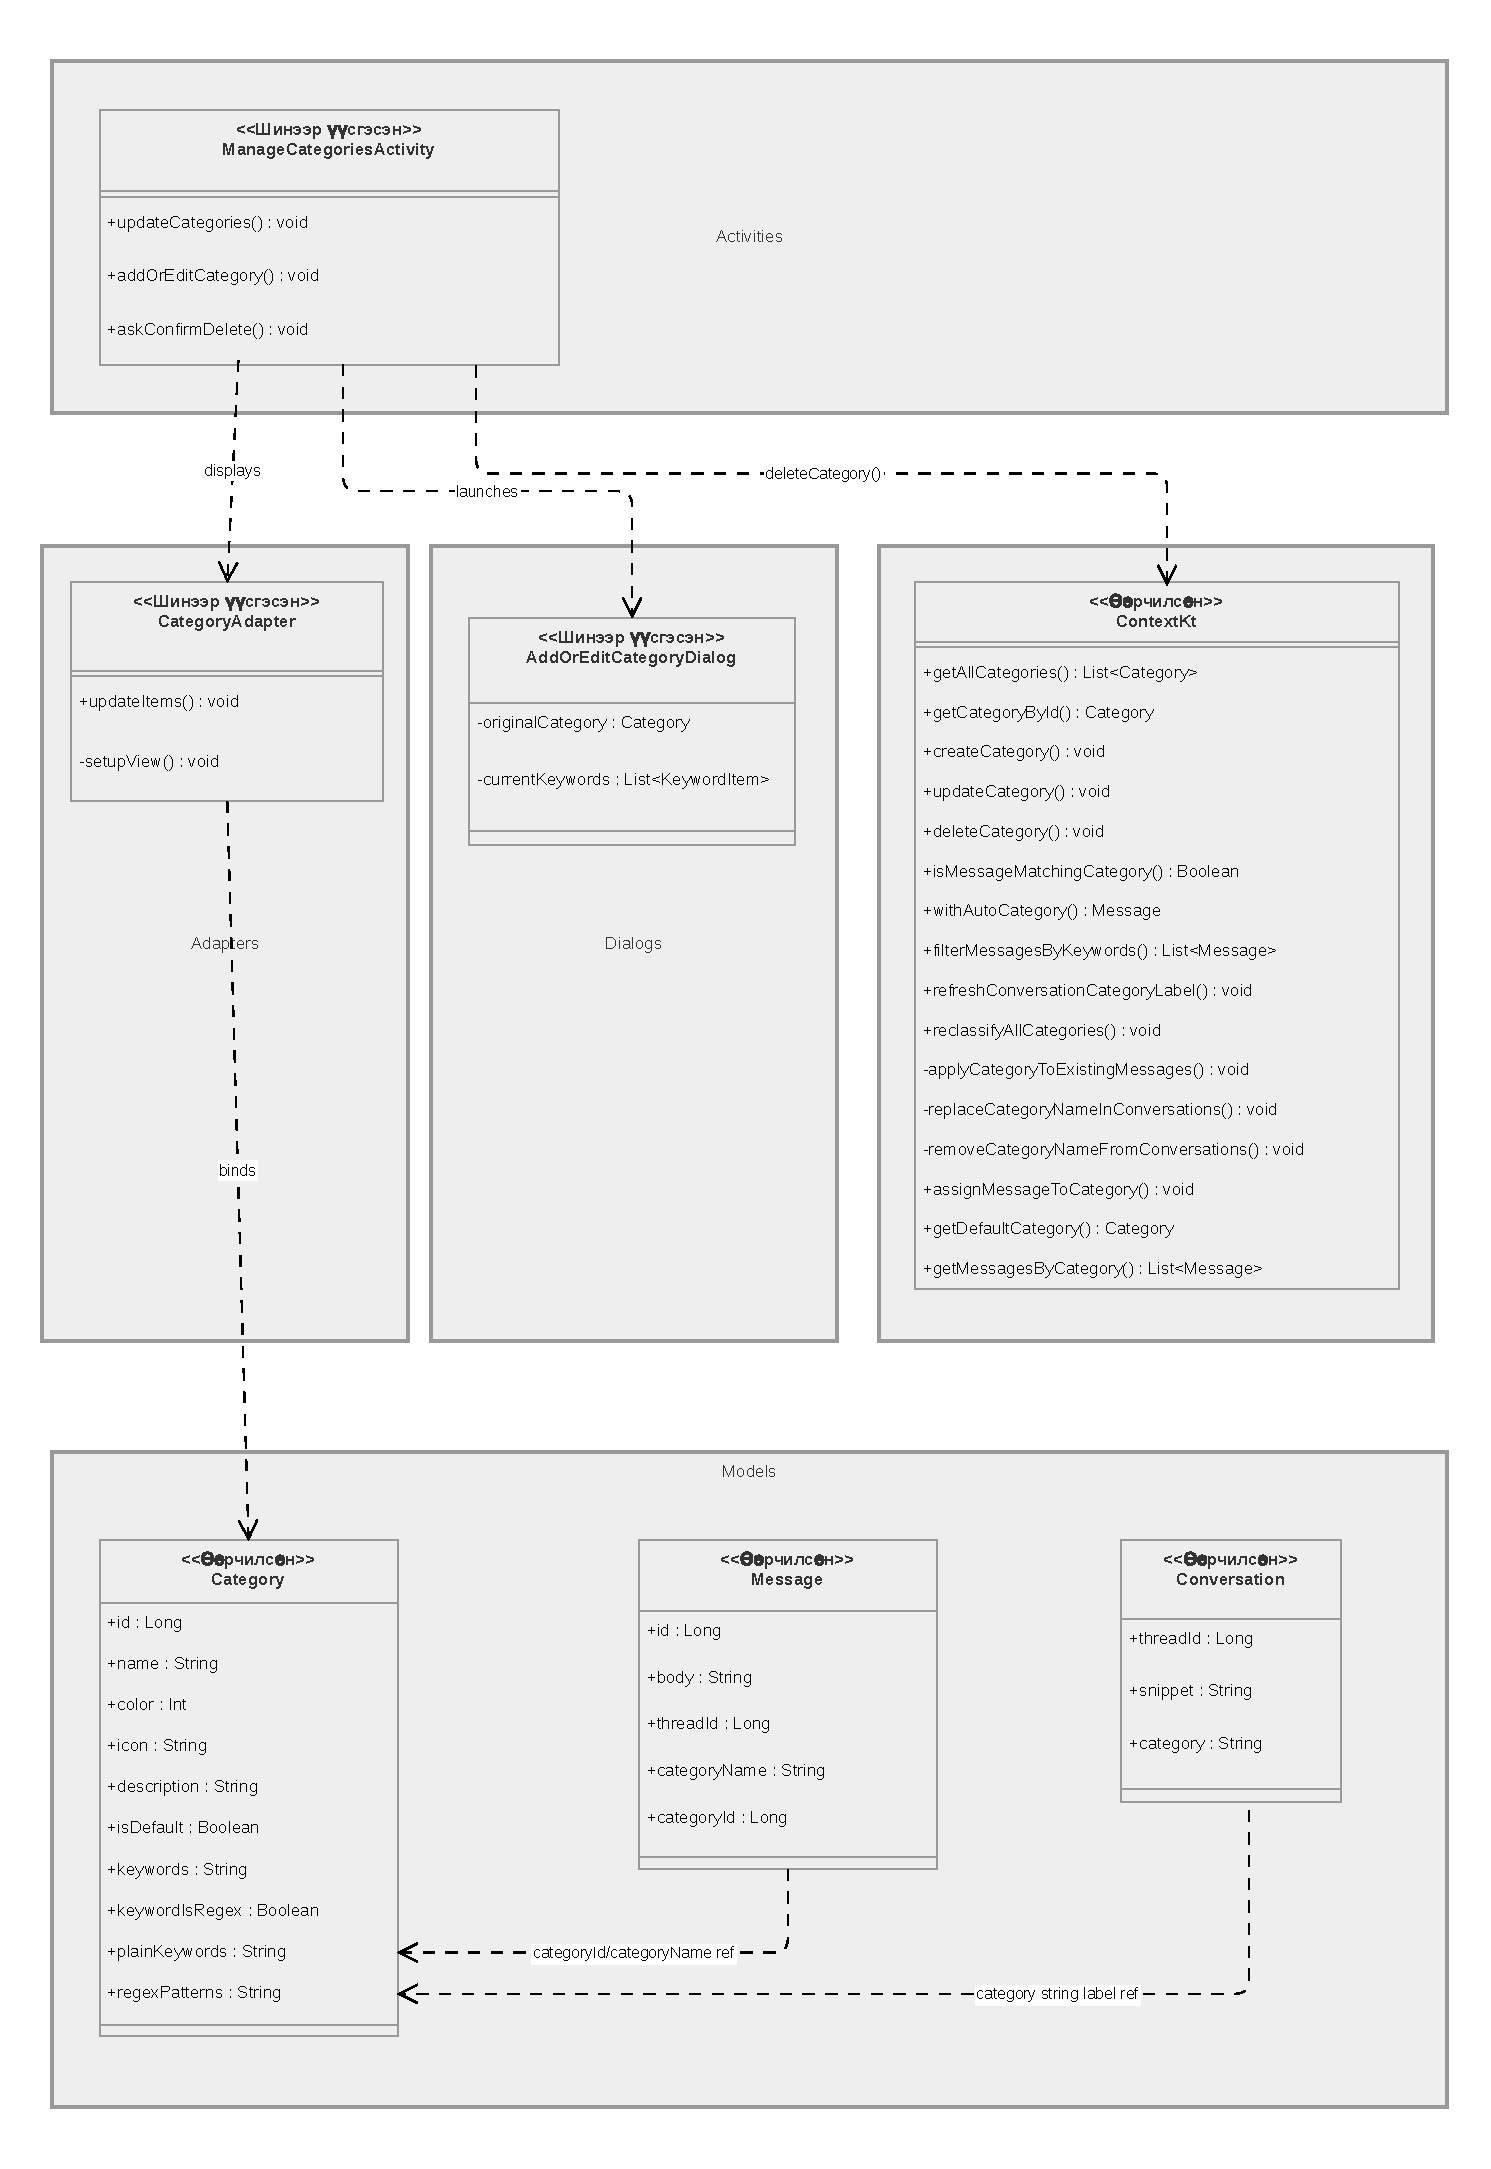
\includegraphics[width=0.85\textwidth]{Diagrams/class/activity}
    \caption{Үндсэн Activity, Fragment болон UI логикийн класс диаграмм}
    \label{fig:class_activity}
\end{figure}

\noindent \textbf{Гол классуудын үүрэг:}
\begin{itemize}
    \item \textbf{ManageCategoriesActivity}: Ангиллын жагсаалтыг шинэчлэх (\texttt{updateCategories}), засах цонх дуудах (\texttt{addOrEditCategory}) үйлдлүүдийг удирдана.
    \item \textbf{MainActivity}: Хадгалсан харагдацуудыг (SavedViewsStore), хугацааны бүлэглэлт (AgeHeaderDecoration), шудрах үйлдэл (inboxSwipeHelper) зэрэг шинэ боломжуудыг нэгтгэсэн.
    \item \textbf{ContextKt}: Системийн бизнес логикийн гол цөм бөгөөд \texttt{withAutoCategory()}, \texttt{refreshConversationCategoryLabel()}, \texttt{filterMessagesByKeywords()} зэрэг өргөтгөл функцүүдийг агуулна.
\end{itemize}

\subsection{Ангилал болон шүүлтүүрийн системийн бүтэц}
Зурвас таних, ангилал үүсгэх болон өгөгдлийн сангийн харилцан хамаарлыг Зураг~\ref{fig:class_category}-д үзүүлэв.

\begin{figure}[H]
    \centering
    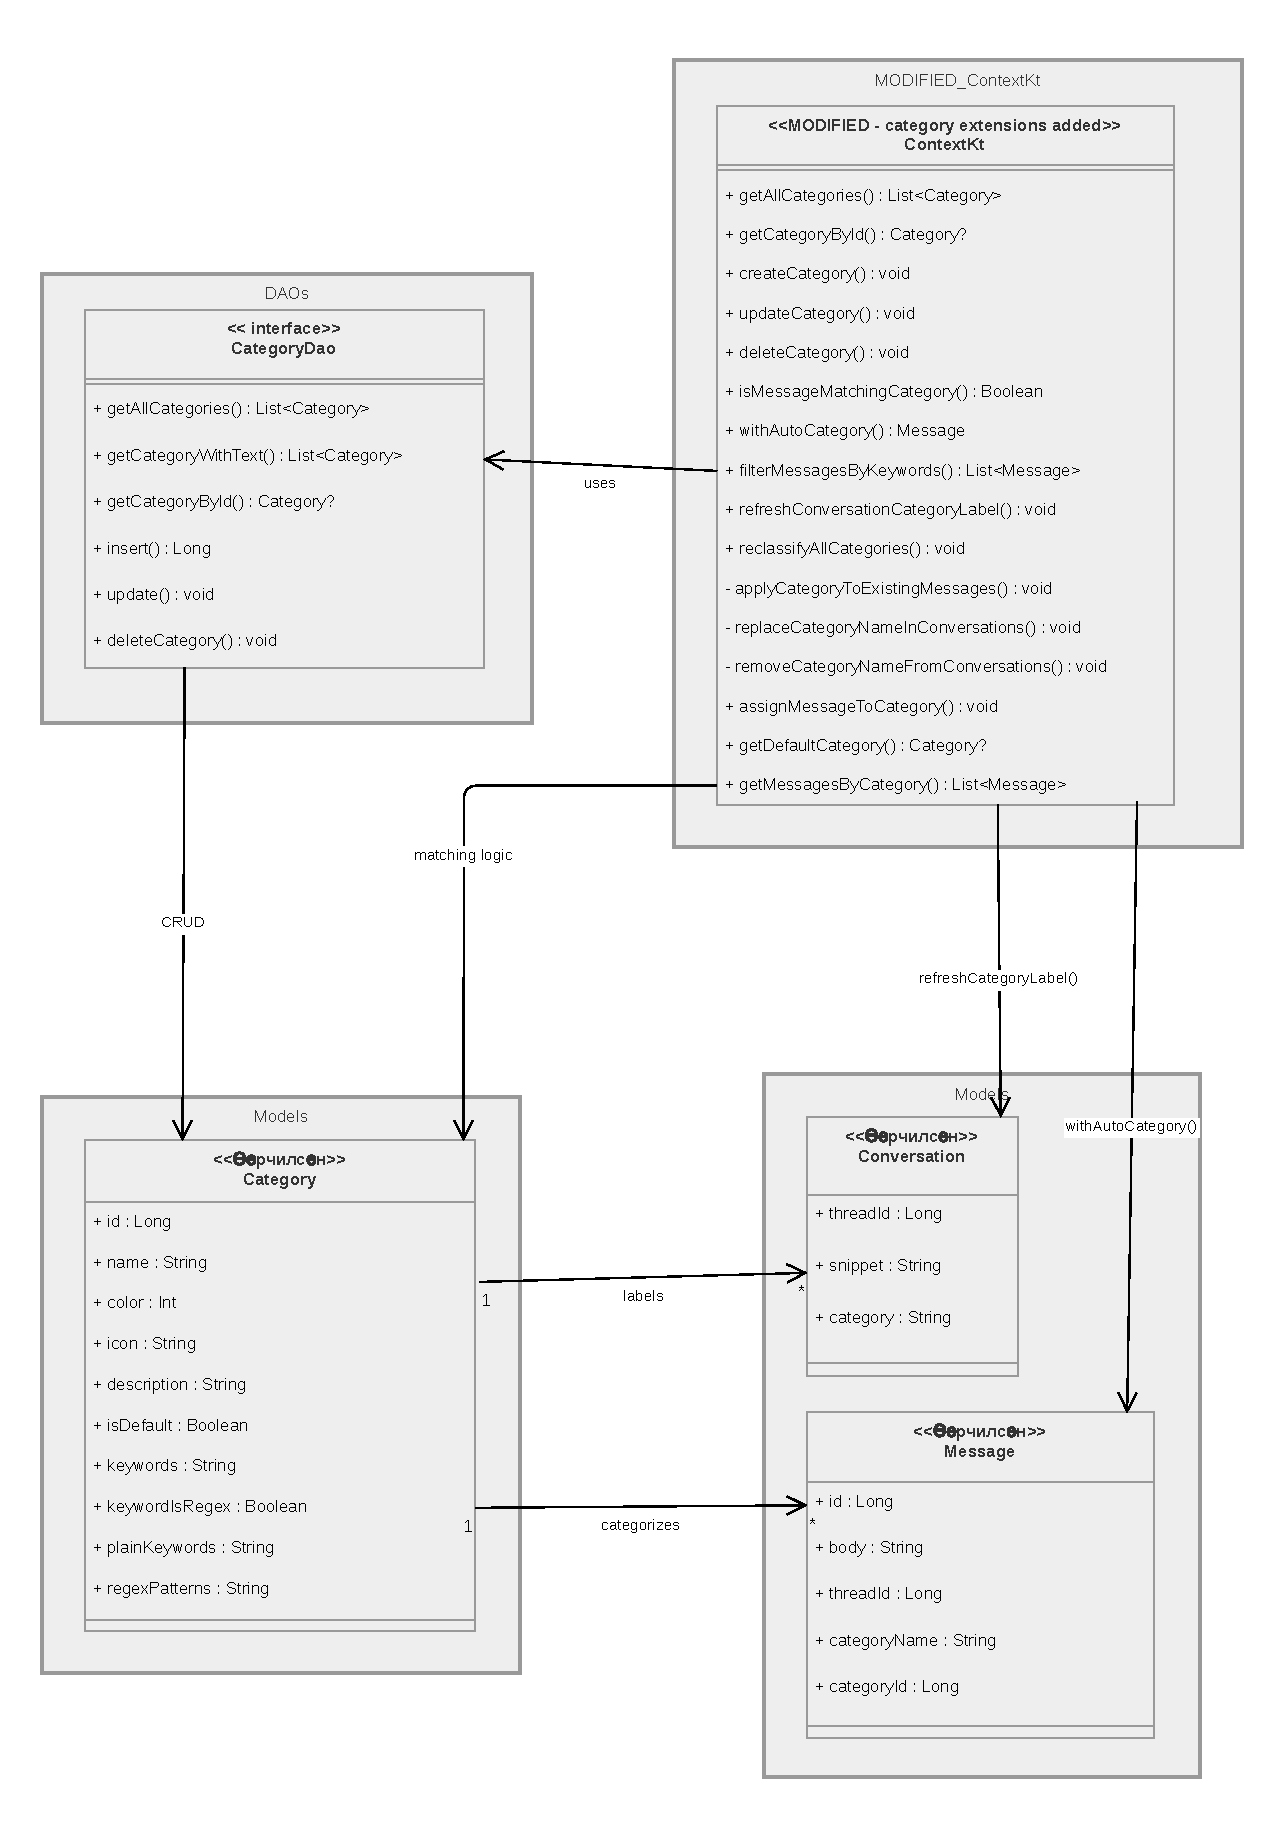
\includegraphics[width=0.85\textwidth]{Diagrams/class/category}
    \caption{Ангилал болон шүүлтүүрийн нарийвчилсан класс диаграмм}
    \label{fig:class_category}
\end{figure}

\noindent \textbf{Бүрэлдэхүүн хэсгүүдийн тайлбар:}
\begin{itemize}
    \item \textbf{CategoryDao}: Ангиллын жагсаалт авах (\texttt{getAllCategories}), түлхүүр үгээр хайх (\texttt{getCategoryWithText}) болон CRUD үйлдлүүдийг гүйцэтгэнэ.
    \item \textbf{Category загвар}: \texttt{plainKeywords} болон \texttt{regexPatterns} талбаруудыг ашиглан ``Dual-mode'' шүүлтүүрийг дэмжинэ.
    \item \textbf{Message загвар}: \texttt{categoryId} болон \texttt{categoryName} талбараар дамжуулан \texttt{Category} загвартай холбогдоно.
\end{itemize}

\subsection{Түлхүүр үгсийн удирдлагын систем ба Compose зохиомж}
Ангиллын дүрмүүдийг удирдах хэрэглэгчийн харилцах цонхны бүтцийг Зураг~\ref{fig:class_ui}-д үзүүлэв.

\begin{figure}[H]
    \centering
    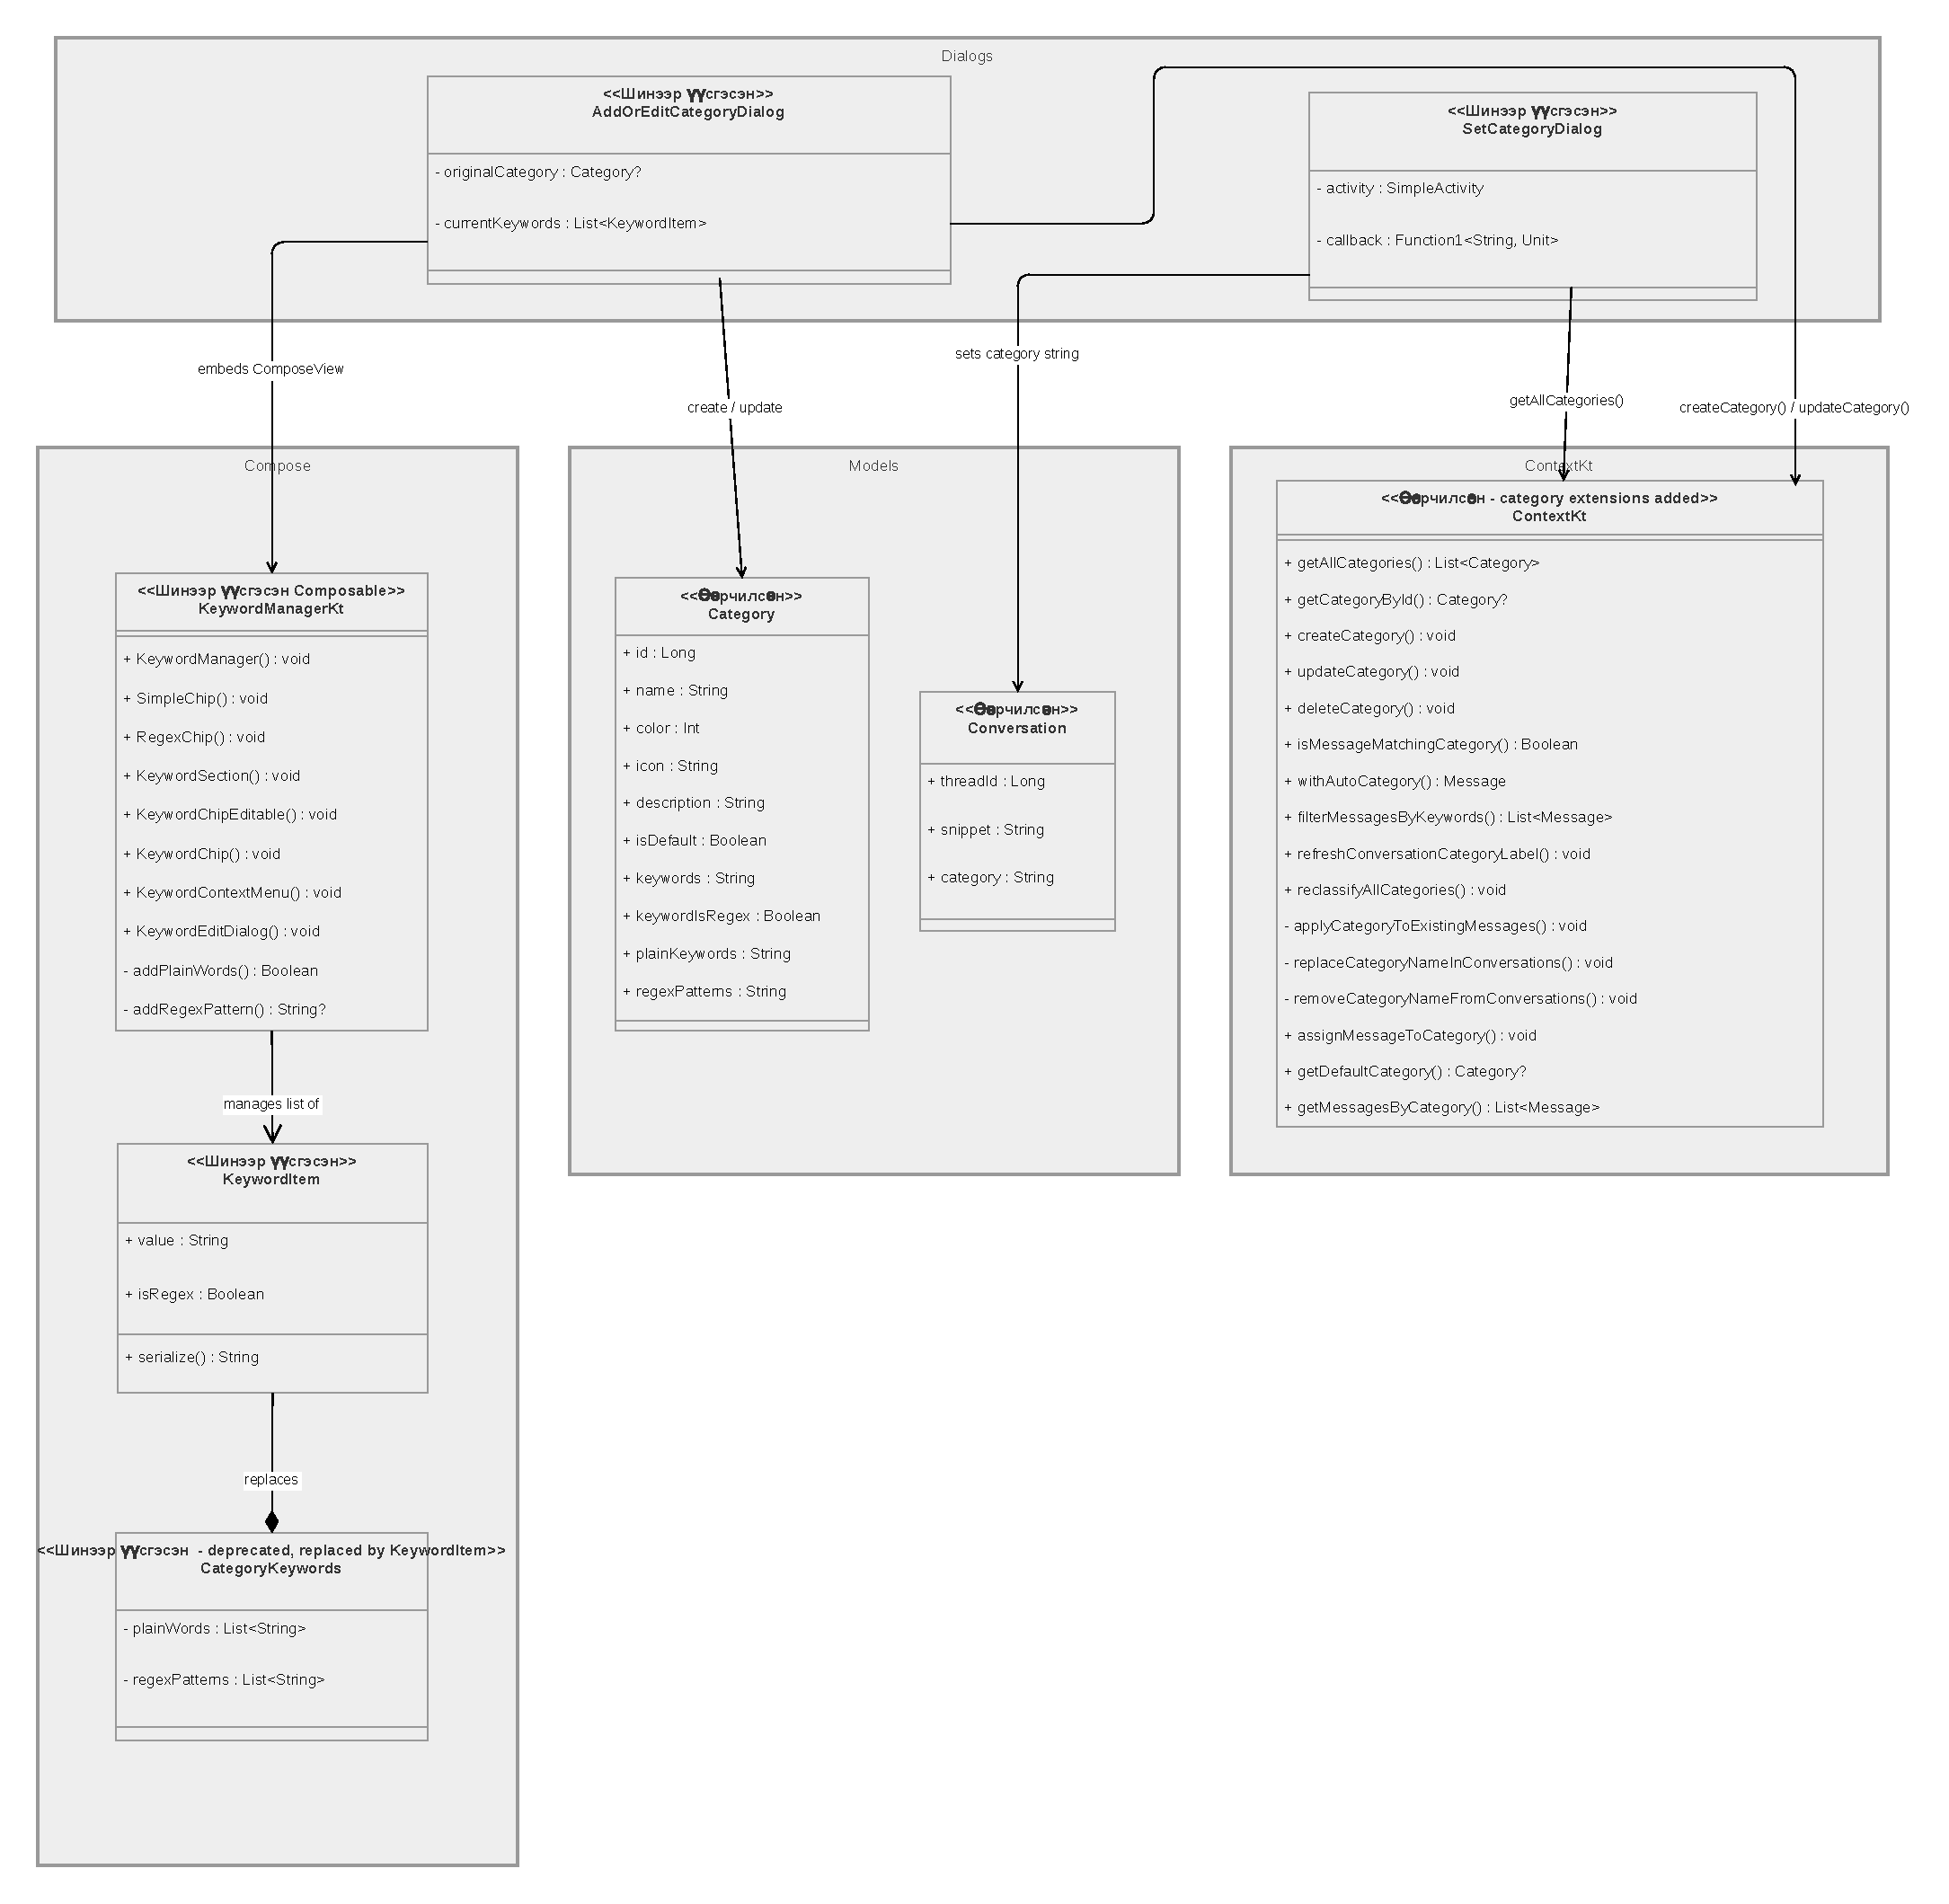
\includegraphics[width=0.85\textwidth]{Diagrams/class/keyboard_ui}
    \caption{Түлхүүр үг удирдах хэрэглэгчийн харилцах цонх болон Compose компонентуудын класс диаграмм}
    \label{fig:class_ui}
\end{figure}

\begin{itemize}
    \item \textbf{KeywordManagerKt}: Түлхүүр үгсийн удирдлагын үндсэн Composable класс. Чип хэлбэртэй харагдацууд (\texttt{SimpleChip}, \texttt{RegexChip}), засах цонх болон контекст цэсийг агуулна.
    \item \textbf{AddOrEditCategoryDialog}: Уламжлалт View систем болон Compose-ийг нэгтгэсэн гүүр. \texttt{createCategory()} болон \texttt{updateCategory()} функцүүдийг дуудаж өгөгдлийг хадгална.
\end{itemize}

% ============================================================
% Section 7: UI/UX зохиомж
% ============================================================
\section{Хэрэглэгчийн харилцах цонхны зохиомж}
Хэрэглэгчийн харилцах цонхыг Material Design 3 стандартын~\cite{material_design} дагуу зохиомжилсон.
\begin{itemize}
    \item \textbf{Adaptive Layout}: Нугалдаг төхөөрөмж нээгдэх үед WindowInfoTracker ашиглан дэлгэцийн талбайг мэдэрч, хоёр баганат харагдац руу автоматаар шилжинэ.
    \item \textbf{Хадгалсан харагдац}: Хавтас тус бүрт өөрийн гэсэн өнгө оноож, харилцан ярианы жагсаалтыг тухайн өнгөөр харуулна.
    \item \textbf{Keyword Manager}: Тогтмол илэрхийлэл болон түлхүүр үгсийг нэг дороос удирдах боломжтой интерактив цонхыг Jetpack Compose-оор хэрэгжүүлсэн.
\end{itemize}

Доод цэсийг эрхий хурууны идэвхтэй бүсэд байрлуулах нь нэг гараар ашиглах эргономикийг сайжруулж \cite{hurff2016thumb}, шудрах үйлдлүүдээр архивлах, уншсан төлөв солих, хавтас оноох зэрэг үйлдлийг нэг алхамд гүйцэтгэх боломж бүрдүүлсэн.

% ============================================================
% Section 8: Аюулгүй байдлын зохиомж
% ============================================================
\section{Аюулгүй байдлын зохиомж}
Хэрэглэгчийн хувийн зурвасын нууцлалыг хангах үүднээс дараах арга хэмжээнүүдийг зохиомжид тусгав:
\begin{itemize}
    \item \textbf{On-device Filtering}: Зурвасыг ангилах бүх процесс зөвхөн төхөөрөмж дээр локал байдлаар хийгдэх бөгөөд гадны сервер рүү өгөгдөл дамжуулахгүй.
    \item \textbf{Local-first Database}: Өгөгдлийн сан нь Android-ийн App Sandbox \cite{android_app_sandbox} дотор тусгаарлагдсан тул бусад аппликейшн шууд хандах боломжгүй.
\end{itemize}
